\chapter{Decomposing mutation and selection to identify mismatched codon usage}
\label{ch:kluyveri}

\clearpage
\pagebreak

This chapter is a lightly revised version of a paper to be submitted to Genome Biology and Evolution and co-authored with Michael A. Gilchrist and Russel Zaretzki.\\
\newline
\newline
C. Landerer, R. Zaretzki, M.A. Gilchrist, Decomposing mutation and selection to identify mismatched codon usage

\section{Abstract}
For decades, codon usage has been used as a measure of adaptation for translational efficiency of a gene's coding sequence.
These patterns of codon usage reflect both the selective and mutational environment in which the coding sequences evolved. %could replace with 'cellular selective and ...'
Over this same period, gene transfer between lineages has become widely recognized as an important biological pheonmena.
Nevertheless, most studies of codon usage implicitly assume that all genes within a genome evolved under the same selective and mutational environment, an assumption violated when introgression occurs. %replace
% could replace 'selective and mutational' with 'cellular;
In order to better understand the effects of introgression on codon usage patterns and vice versa,  we examine the patterns of codon usage in the yeast which has experienced a large introgression, \textit{Lachancea kluyveri}.
%The \kluyveri genome provides an opportunity to study the evolution of introgressed genes to a novel cellular environment and estimate the fitness cost such a transfer imposes.
We quantify the effects of mutation bias and selection for translation efficiency on the codon usage pattern of the endogenous and introgressed exogenous genes using a Bayesian mixture model, \ROC, which is built on mechanistic assumptions of protein synthesis and grounded in population genetics.
We find substantial differences in codon usage between the endogenous and exogenous genes, and show that these differences can be largely attributed to a shift in mutation bias from A/T ending codons in the endogenous genes to C/G ending codons in the exogenous genes.
Recognizing the two different signatures of mutation and selection bias improves our ability to predict protein synthesis rate by $17 \%$ and allowed us to accurately assess codon preferences.
In addition, using our estimates of mutation and selection bias, we to identify \textit{Eremothecium gossypii} as the most likely source lineage, estimate the introgression occurred $\sim 6\times 10^8$ generation ago, and estimate its historic and current genetic load.
Together, our work illustrates the advantage of mechanistic, population genetic models like \ROC and the quantitative estimates they provide when analyzing sequence data.

\newpage


\section{Introduction}
Synonymous codon usage patterns varies within a genome and between taxa, reflecting differences in mutation bias, selection, and genetic drift.
The signature of mutation bias is largely determined by the organism's internal or cellular environment, such as their DNA repair genes or UV exposure.
While this mutation bias is an omnipresent evolutionary force, its impact can be obscured or even amplified by selection. 
The signature of selection on codon usage is also largely determined by an organism's cellular environment, such as its tRNA species, their copy number, and post-transcriptional modifications.
The strength of selection on the codon usage of an individual gene is largely determined by its expression level which, in turn, is also largely determined by the organism's external environment.
In general, the strength of selection on codon usage increases with its expression level \citep{gouy1982, ikemura1985, bulmer1990}, specifically its protein synthesis rate \citep{gilchrist2007}.
Thus as gene expression increases, codon usage shifts from a process dominated by mutation to a process dominated by selection.
The overall efficacy of selection on codon usage is a function of the organism's effective population size $N_e$ which, in turn, is largely determined by its external environment.
By explicitly modeling the combined forces of mutation, selection, and drift, \ROC allows us disentangle the evolutionary forces responsible for the patterns of codon usage bias (CUB) encoded in an species' genome \citep{gilchrist2007, ShahAndGilchrist2011, wallace2013, gilchrist2015}, should provide biologically meaningful information about the lineage's historical cellular and external environment.

Most studies implicitly assume that the CUB of a genome is shaped by a single cellular environment. 
As genes are horizontally transferred, introgress, or combined to form novel hybrid species, one would expect to see the influence of multiple cellular environments on a genomes codon usage pattern \citep{medigue1991,lawrence1997}.
Given that transferred genes are likely to be less adapted than endogenous genes to their new cellular environment, we expect a greater fitness burden of transferred genes if donor and recipient environment differ greatly in their selection bias, making such transfers less likely.
More practically, if differences in codon usage of transferred genes are unaccounted for, they may distort parameter estimates.
Such distortion could lead to the wrong codon preference for an amino acid, underestimate the variation in protein synthesis rate, or bias mutation estimates when analyzing a genome.

To illustrate these ideas, we analyze the CUB of the genome of \emph{Lachancea kluyveri}, the earliest diverging lineage of the Lachancea clade.
The Lachancea clade diverged from the Saccharomyces clade, prior to its whole genome duplication $\sim 100$ Mya ago \citep{MHM2015,Beimforde2014}.
Since that time, \kluyveri has experienced a large introgression of exogenous genes found in all populations \citep{friedrich2015}.
The introgression replaced the left arm of the C chromosome and displays a $13 \%$ higher \GC than the endogenous \kluyveri genome \citep{payen2009, friedrich2015}.
These characteristics make \kluyveri an ideal model to study the effects of an introgressed cellular environment and the resulting mismatch in codon usage.

Using \ROC, a Bayesian population genetics model based on a mechanistic description of ribosome movement along an mRNA, allows us to quantify the cellular environment in which genes have evolved by separately estimating the effects of mutation bias and selection bias on codon usage.
\ROC's resulting predictions of protein synthesis rates have been shown to be on par with laboratory measurements \citep{ShahAndGilchrist2011, gilchrist2015}.
We use \ROC to independently describe two cellular environments reflected in the \kluyveri genome; the signature of the current environment in the endogenous genes and the decaying signature of the exogenous environment in the introgressed genes.
Our results indicate that the difference in \GC between endogenous and exogenous genes is mostly due to the differences in mutation bias of their ancestral environments.
Accounting for these different signatures of mutation bias and selection bias of the endogenous and exogenous sets of genes substantially improves our ability to predict present day protein synthesis rates.
These endogenous and exogenous gene set specific estimates of mutation bias and selection bias, in turn allow us to address more refined questions of biological importance.
For example, it allows us to identify \gossypii as the most likely source of the introgressed genes out of the 38 yeast lineages with sequenced genomes, estimate the age of the introgression to be on the order of 0.2-1 Mya, estimate the genetic load of these genes, both at the time of introgression and now, as well as make predictions about how the CUB of the introgressed genes will evolve in the future.

%For example, of 38 sequenced yeast lineages, we identified the most likely source lineage of the exogenous genes using a combination of information in codon usage and gene synteny.
%We compared estimates of mutation bias (\DM) and selection bias (\DE) for the exogenous genes to each yeast lineage and further investigated candidate lineages using synteny.
%This allows us to identify \gossypii as the most likely source of the introgressed genes.
%Next, we estimate the time since introgression and the persistence of the signal of the exogenous cellular environment from our estimates of \DM using an exponential model of decay.
%We estimate the age of the introgression to be on the order of 0.2-1 Mya.
%Third, we estimate the selective cost of the mismatched codon usage for the introgression, using our estimates of \DE and protein synthesis rate $\phi$.
%This allows us to hypothesize about the genetic load of these genes, both at the time of introgression and now, as well as make predictions about the codon usage the introgressed genes will evolve in the future.

\section{Results}
\subsection{The Signatures of two Cellular Environments within \kluyveri's Genome}
We used our software package AnaCoDa \citep{landerer2018} to compare model fits of \ROC to the entire \kluyveri genome and its genome partitioned into two sets of 4,864 endogenous and 497 exogenous genes.
AIC values strongly support the hypothesis that the \kluyveri genome consists of genes with two different and distinct patterns of codon usage bias ($\Delta\text{AIC} = 75,462$; Table \ref{tab:AIC}).
We find additional support for this hypothesis when we compare our predictions of gene expression to empirically observed values.
Specifically, the explanatory power between our predictions and observed values improved by $\sim 42\%$, from $R^2 = 0.33$ to $0.46$ (Figure \ref{fig:phi_corr_two_cond}).

\begin{table}[h]
  \centering
  \caption{Model selection of the two competing hypothesis. 
  Reported are the log-likelihood, $\log(\Lik)$, the number of parameters estimated $n$, AIC, and $\Delta$AIC values.}
  \begin{tabular}{lrrrr}
    \hline
    Hypothesis             & $\log(\Lik)$ &$n$ &  AIC & $\Delta$AIC\\ \hline 
    Separated		   & -2,612,397 & 5,402 & 5,235,598&      0\\
    Combined               & -2,650,047 & 5,483 & 5,311,060& 75,462\\ \hline
  \end{tabular}
  \label{tab:AIC_klu}
\end{table}
\clearpage

\begin{figure}
    \centering
    \begin{subfigure}
        \centering
        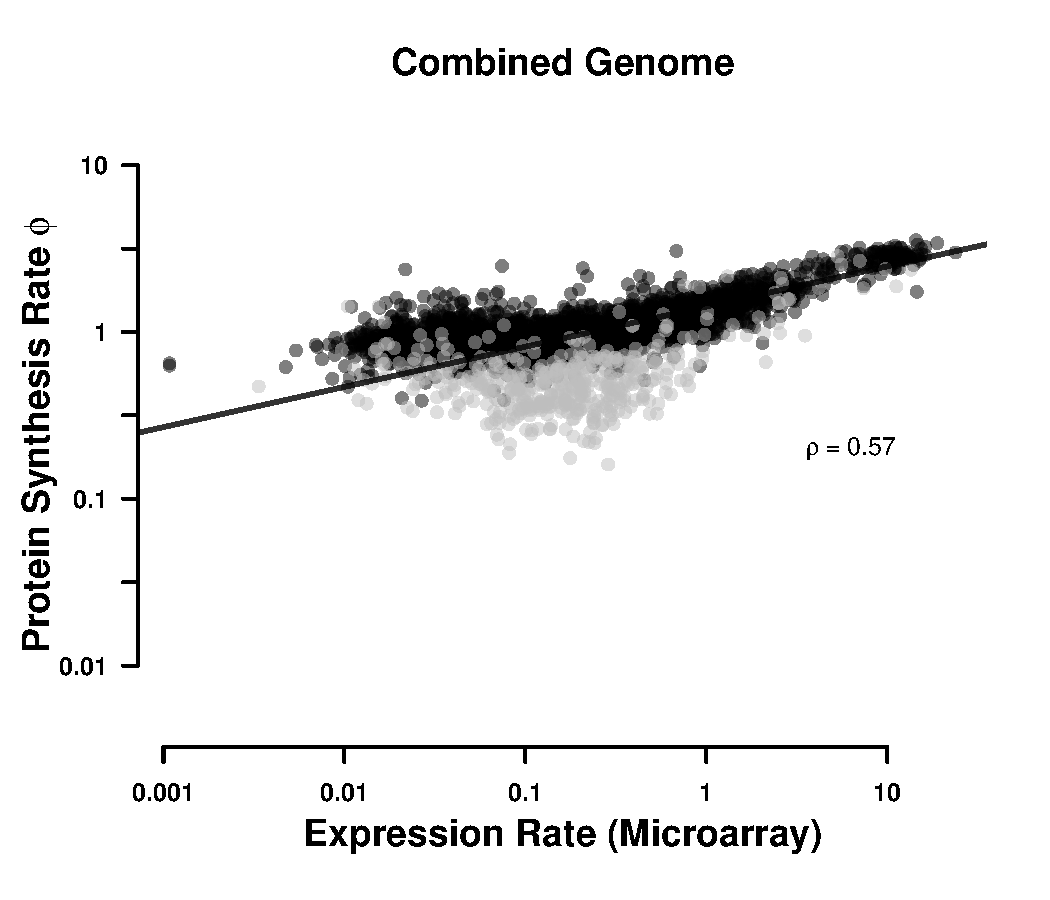
\includegraphics[width=.45\textwidth]{ch3/phi_corr_plot_whole_Genome_estim.pdf}
    \end{subfigure}
    \begin{subfigure}
        \centering
        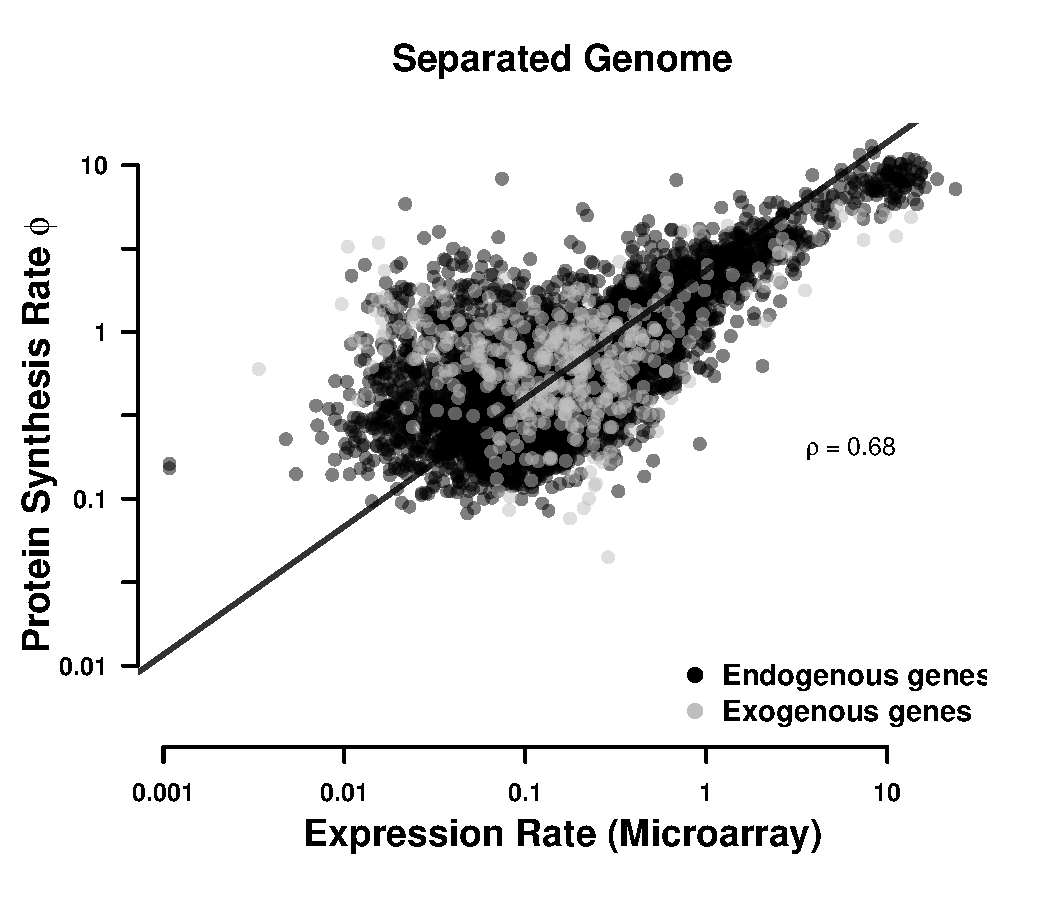
\includegraphics[width=.45\textwidth]{ch3/phi_corr_plot_split_Genome_estim.pdf}
    \end{subfigure}
    \caption{Comparison of predicted protein synthesis rate $\phi$ to microarray data from \citet{tsankov2010} for (a) the combined genome and (b) the separated endogenous and exogenous genes. 
    Endogenous genes are displayed in black and exogenous genes in red. Black line indicates type II regression line \cite{SokalAndRohlf1981}.}
    \label{fig:phi_corr_two_cond}
\end{figure}


\subsection{Comparing Differences in the Endogenous and Exogenous Codon Usage}
To better understand the differences in the endogenous and exogenous cellular environments, we compared our parameter estimates of mutation bias \DM and selection \DE for the two sets of genes.
Our estimates of \DM for the endogenous and exogenous genes were negatively correlated ($\rho = -0.49$),  indicating weak concordance of $\sim5\%$ between the two mutation environments (Figure \ref{fig:csp_comp}).
For example, the endogenous genes show a mutational preference for A and T ending codons in $\sim95\%$ of the codon families.
In contrast, the exogenous genes display an equally consistent mutational preference towards C and G ending codons (Table \ref{tab:codon_pref_dm}).
As a result, only the two codon amino acid Phenylalanine (Phe, F) shares the same rank order across the endogenous and exogenous \DM estimates.

\begin{figure}
    \centering
    \begin{subfigure}
        \centering
        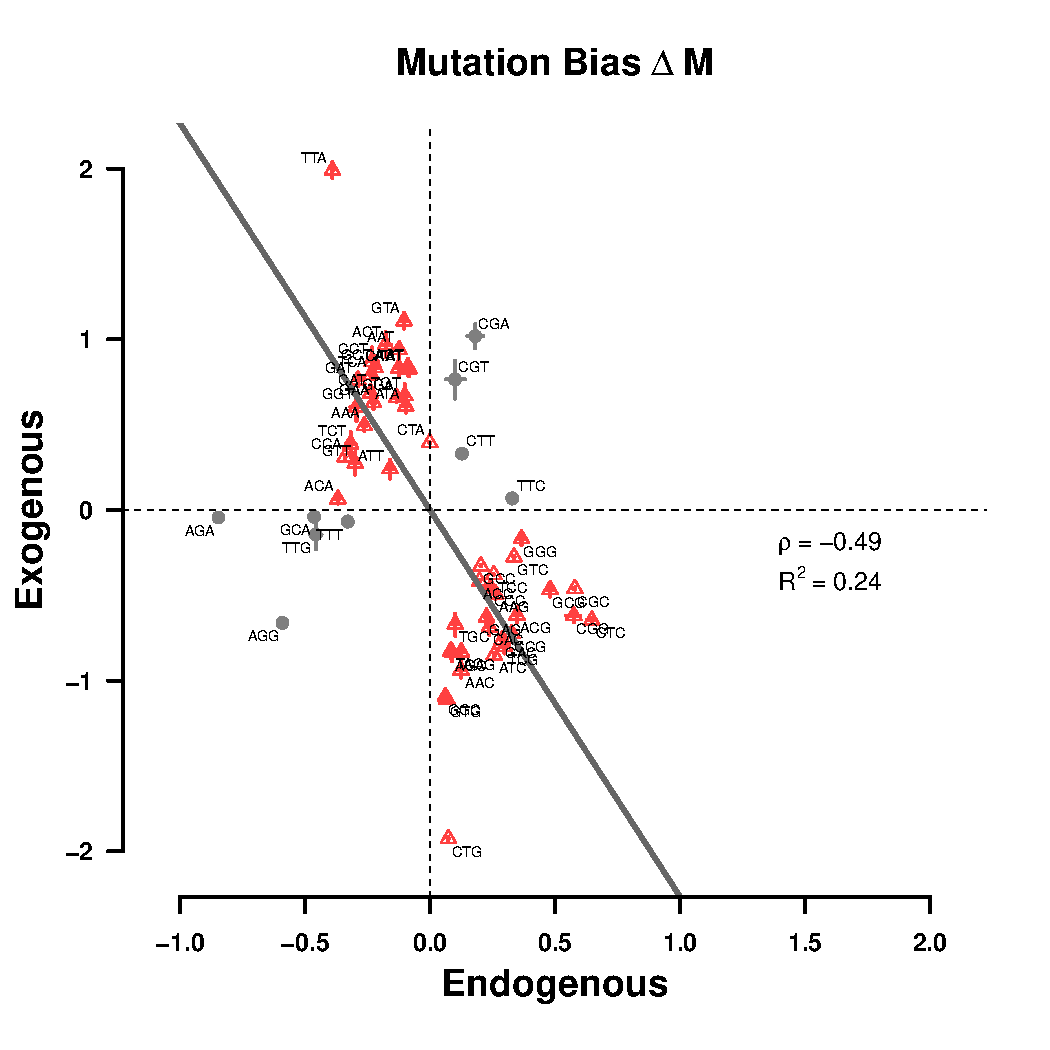
\includegraphics[width=.45\textwidth]{ch3/csp_corr_dm.pdf}
    \end{subfigure}
    \begin{subfigure}
        \centering
        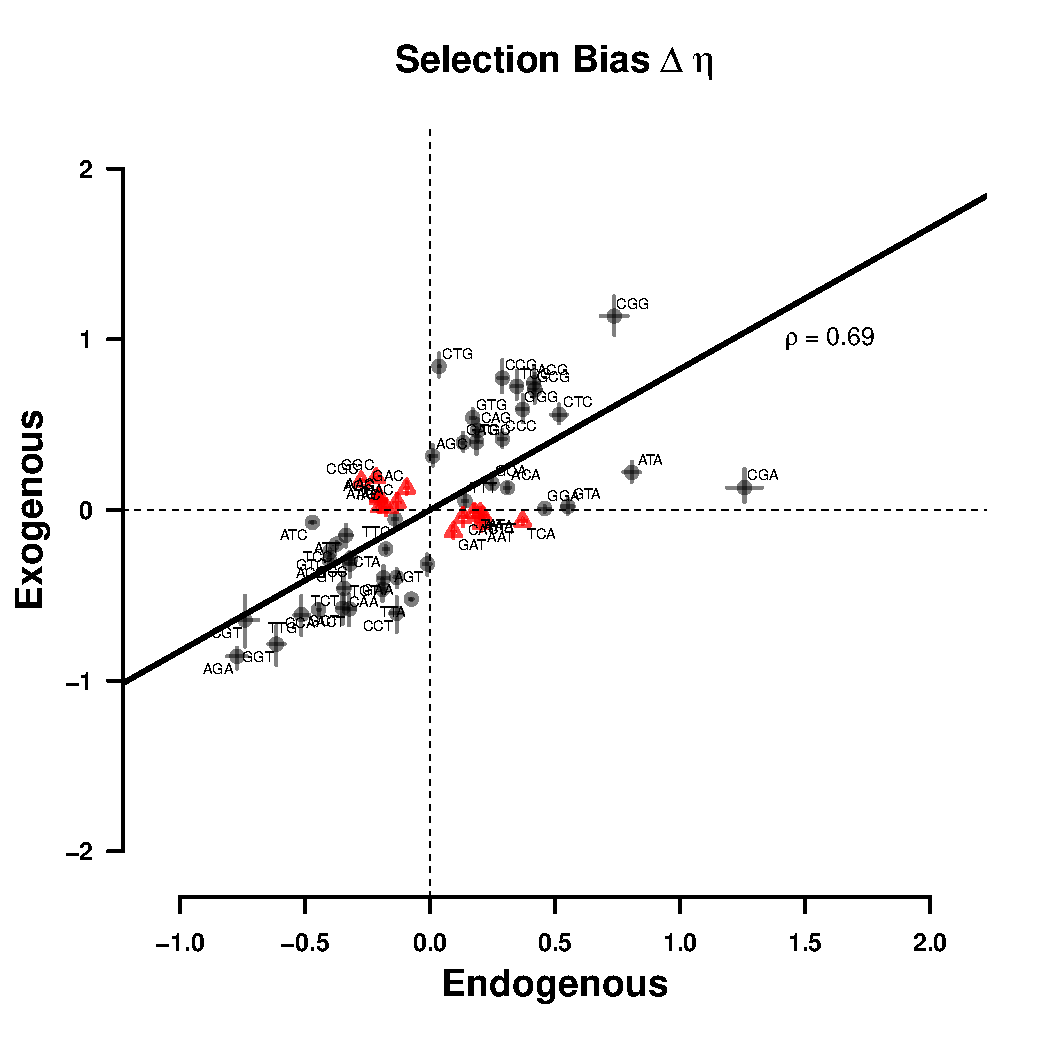
\includegraphics[width=.45\textwidth]{ch3/csp_corr_deta.pdf}
    \end{subfigure}
    \caption{Comparison of (a) mutation bias \DM and (b) selection bias \DE parameters for endogenous and exogenous genes.
      Estimates are relative to the mean for each codon family.
      Black dots indicate \DM or \DE parameters with the same sign for the endogenous and exogenous genes, red dots indicate parameters with different signs.
      Black line shows the type II regression line \citep{SokalAndRohlf1981}.
      Dashed lines mark quadrants.}
    \label{fig:csp_comp}
\end{figure}

In contrast, our estimates of \DE for the endogenous and exogenous genes were positively correlated ($\rho = 0.69$) and showing concordance of $\sim53\%$ between the two selection environments (Figure \ref{fig:csp_comp}).
We find that the strength of selection within each codon family differs between sets of genes.
Overall, the endogenous genes only show a selection preference for C and G ending codons in $\sim58\%$ of the codon families.
In contrast, the exogenous genes display a strong preference for A and T ending codons in $\sim89\%$ of the codon families.

The difference in codon usage between endogenous and exogenous genes is striking.
As a result, our estimates of the optimal codon differ in nine cases between endogenous and exogenous genes (Table \ref{tab:codon_pref_deta}).
Fits to the complete \kluyveri genome reveal that the relatively small exogenous gene set ($\sim 10\%$ of genes) has a disproportional effect on the model fit.
We find that the complete \kluyveri genome is estimated to share the mutational preference with the exogenous genes in $\sim78\%$ of the $19$ codon families that are discordant between the endogenous and exogenous genes.
In two cases, Isoleucine (Ile, I) and Arginine (Arg, R), the strong discordance in mutation preference results in an estimated codon preference in the complete \kluyveri genome that differs from both the endogenous, and the exogenous genes.

The effect of the small exogenous gene set on the fit to the complete \kluyveri genome is smaller in our estimates of selection bias \DE than \DM, but still large.
We find that the complete \kluyveri genome is estimated to share the selection preference with the exogenous genes in $\sim60\%$ of codon families that show discordance between endogenous and exogenous genes.
These results clearly show that it is important to recognize the difference in endogenous and exogenous genes and treat these genes as separate sets to avoid the inference of incorrect synonymous codon preferences and better predict protein synthesis.

\subsection{Determining Source of Exogenous Genes}

We combined our estimates of mutation bias \DM and selection bias \DE with synteny information and searched for potential source lineages of the introgressed exogenous region.
We examined 38 yeast lineages (Table \ref{tab:org_overview}) of which two (\emph{Eremothecium gossypii} and \emph{Candida dubliniensis}) showed a strong positive correlation in codon usage (Figure \ref{fig:csp_exo_comp}).
The endogenous \kluyveri genome exhibits codon usage very similar to most yeast lineages examined, indicating little variation in codon usage among the examined yeasts (Figure \ref{fig:csp_endo_comp}).
Four lineages show a positive correlation for $\Delta M$ and $\Delta \eta$ with the exogenous genes and have a weak to moderate positive correlation in selection bias with the endogenous genes; but, like the exogenous genes, tend to have a negative correlation in $\Delta M$ with the endogenous genes.

Comparing synteny between the exogenous genes, which are restricted to the left arm of chromosome C, and \gossypii and \dubl as well as closely related yeast species we find that \gossypii displays the highest synteny (Figures \ref{fig:synt_rel} \& \ref{fig:synteny_species}).
\dubl, even though it displays similar codon usage does not show synteny with the exogenous region.
Furthermore, the synteny relationship between the exogenous region and other yeasts appears to be limited to the Saccharomycetacease clade (Figure \ref{fig:synteny_species}).
Given these results, we conclude that of the 38 examined yeast lineages the \gossypii lineage is the most likely source of the introgressed exogenous genes.

\singlespacing
\begin{figure}
     \centering
	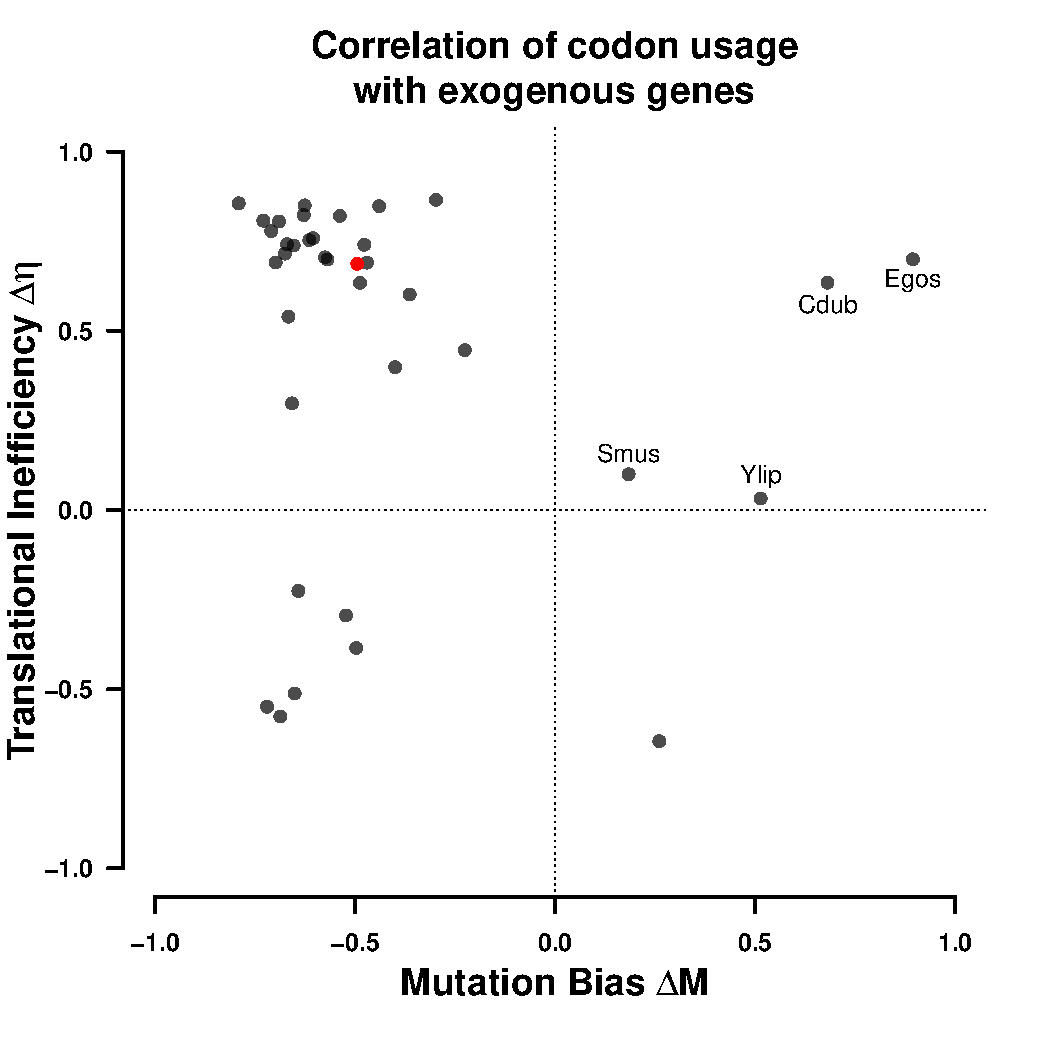
\includegraphics[width=.45\textwidth]{ch3/csp_mean_correlation_exo.pdf}
	\caption{Correlation of \DM and \DE of the exogenous genes with 38 examined yeast lineages. 
	Dots indicate the correlation of \DM and \DE of the lineages with the endogenous and exogenous parameter estimates. 
	All regressions were performed using a type II regression \citep{SokalAndRohlf1981}.}
	\label{fig:csp_exo_comp}
\end{figure}
\doublespacing

\subsection{Estimating Introgression Age}

We modeled the change in codon frequency as a model of exponential decay, we estimated the age of the introgression assuming that \gossypii still represents the mutation bias of its ancestral source lineage at the time of the introgression and a constant mutation rate.
We infer the age of the introgression to be on the order of $6.2\pm1.2\times 10^8$ generations. 
Assuming \kluyveri experiences between one and eight generations per day, we estimate the introgression to have occurred between $212,000$ to $1,700,000$ years ago.
Our estimate places the time of the introgression earlier than previously assumed \citep{friedrich2015}.
%However, our estimates are likely overestimates as they are based on our estimates of mutation bias $\Delta M$ and assume a purely neutral decay of the exogenous cellular environment.

Using the same approach, we also estimated the persistence of the signal of the exogenous cellular environment.
We assume that differences in mutation bias will decay more slowly than differences in selection bias to be able to utilize our bias free estimates of \DM.
We predict that the \DM signal of the source cellular environment will have decayed to be within one percent of the \kluyveri environment in $\sim 5.4\pm0.2\times 10^9 $ generations, or between $1,800,000$ and $15,000,000$ years.
Together, these results indicate that the mutation signature of the exogenous genes will persist for a very long time.

\subsection{Genetic Load due to Mismatching Codon Usage of the Exogenous Genes}

\marginpar{Explicitly mention value for genetic load}
We define genetic load as the difference between the fitness of an expected, replaced endogenous gene and the exogenous gene, $s \propto \phi \DE$ due to the mismatch in codon usage parameters (See Methods for details).
Estimates of selection bias for the exogenous genes show that, while well correlated with the endogenous genes, only nine amino acids share the same optimal codon.
Exogenous genes are, therefore, expected to represent a significant reduction in fitness, or genetic load for \kluyveri due to this mismatch in codon usage.
As the introgression occurred before the diversification of \kluyveri and has fixed throughout all populations \citep{friedrich2015}, we can not observe the original endogenous sequences that have been replaced by the introgression.
Using our estimates of $\Delta M$ and $\Delta \eta$ from the endogenous genes and assuming hat the current exogenous amino acid composition of genes is representative of the replaced endogenous genes, we estimate the genetic load of the exogenous genes at the time of introgression (Figure \ref{fig:sne_fitness_burden}a) and currently (Figure \ref{fig:sne_fitness_burden}b).
We find that the genetic load due to mismatched codon usage was -0.0008 at the time of the introgression and still represents a genetic load of -0.0003 today.

In order to account for differences in the efficacy of selection on codon usage between the donor lineage and \kluyveri using a linear scaling factor $\kappa$ (See Methods for details).
We predict that a small number of low expression genes ($\phi < 1$) were weakly exapted at the time of the introgression (Figure \ref{fig:sne_fitness_burden}a).
High expression genes ($\phi > 1$) are predicted to have carried the largest genetic load in the novel cellular environment.
These highly expressed genes are inferred to have the greatest degree of adaptation since the time of the introgression to the \kluyveri cellular environment (Figures \ref{fig:sne_fitness_burden}a \& \ref{fig:adapt_tot}).

\begin{figure}
    \centering
    \begin{subfigure}
        \centering
        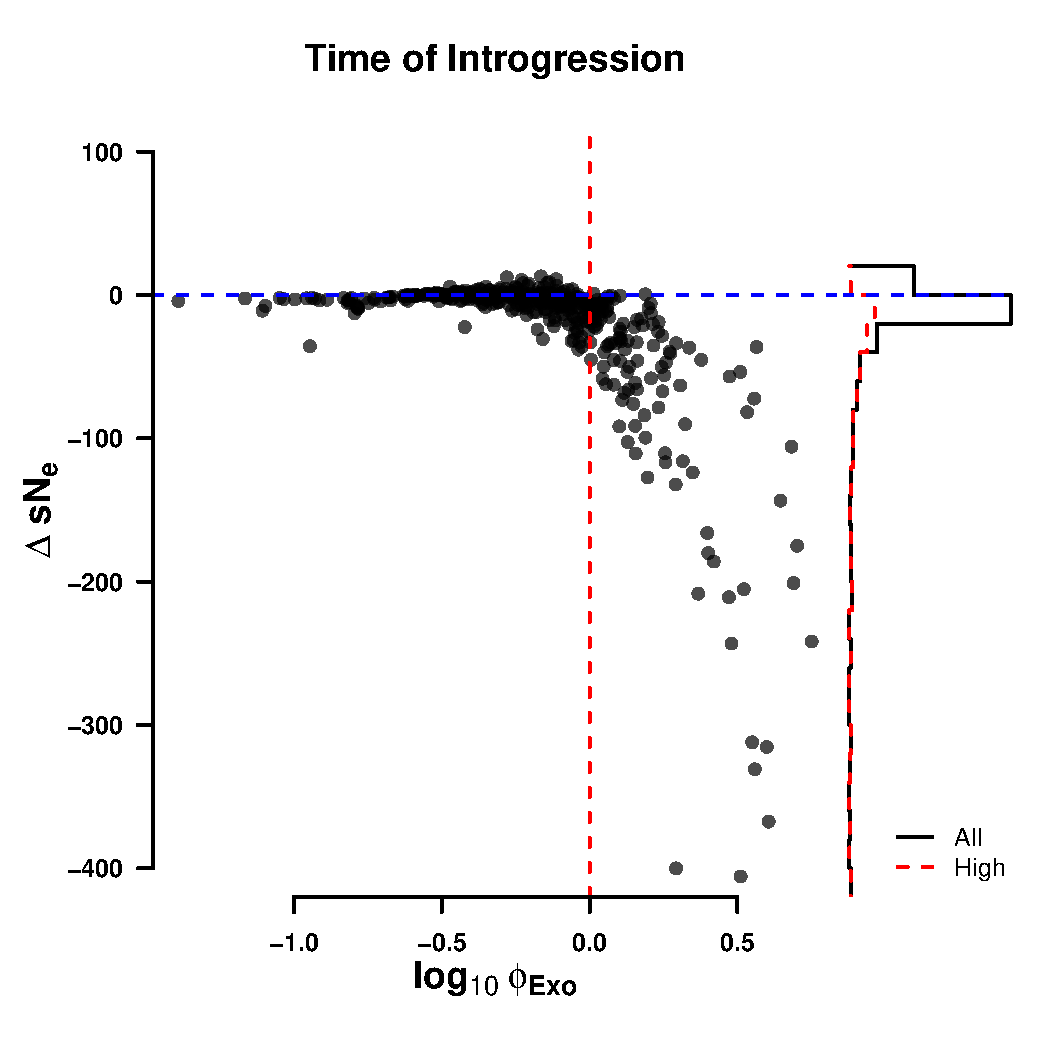
\includegraphics[width=.45\textwidth]{ch3/fitness_difference_gos_kappa5.pdf}
    \end{subfigure}
    \begin{subfigure}
        \centering
        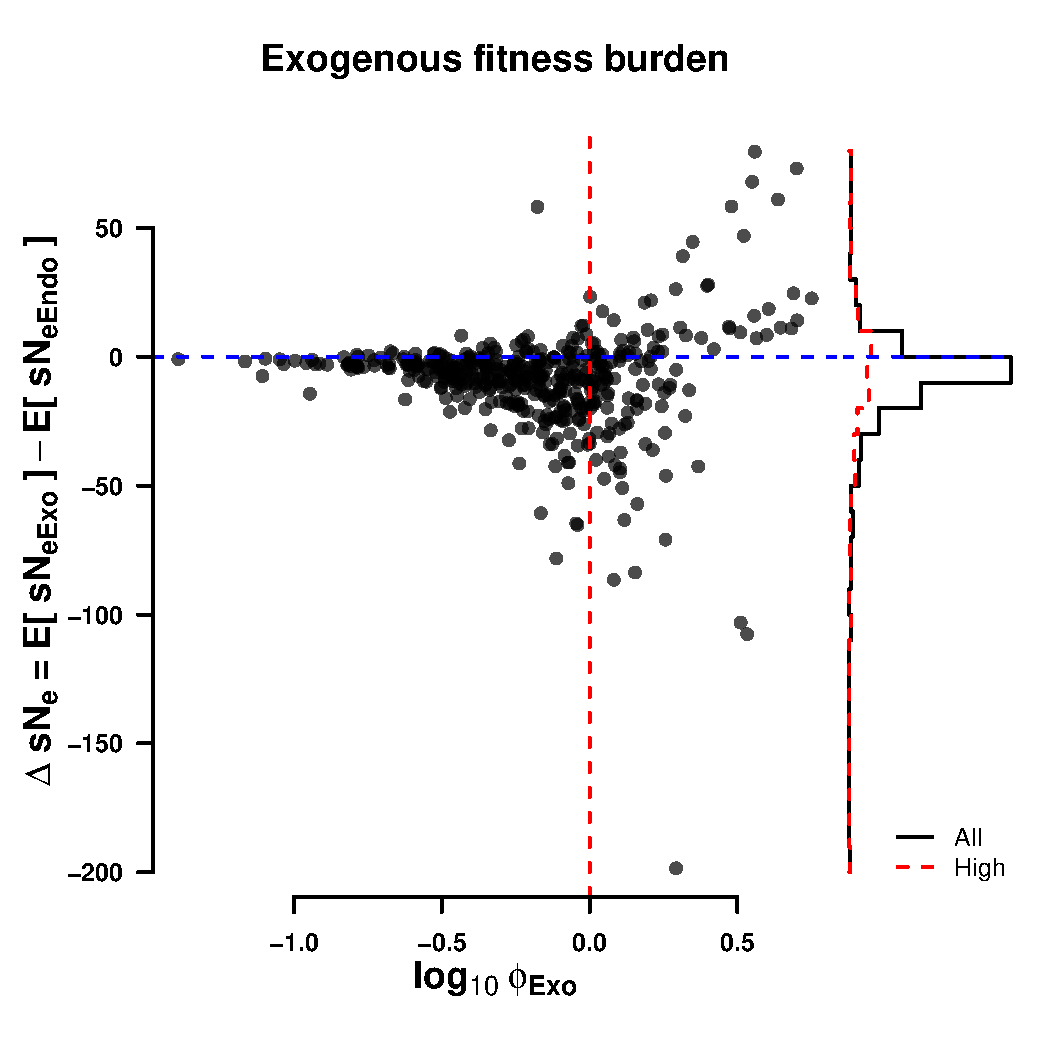
\includegraphics[width=.45\textwidth]{ch3/fitness_difference_exo.pdf}
    \end{subfigure}
    \caption{Genetic load $s = \DE \phi$ (a) at the time of introgression ($\kappa = 5$), and (b) currently ($\kappa = 1$). }
    \label{fig:sne_fitness_burden}
\end{figure}


\section{Discussion}
In order to study the evolutionary effects of an introgression, we used \ROC, a mechanistic model of ribosome movement along an mRNA.
Our parameter estimates indicate that the \kluyveri genome contains distinct signatures of mutation and selection bias from both an endogenous and exogenous cellular environment.
By fitting \ROC separately to \kluyveri's endogenous and exogenous sets of genes we generate a quantitative description of their signatures of mutation bias and natural selection for efficient protein translation.
Our results indicate that the difference in \GC between endogenous and exogenous genes is mostly due to differences in mutation bias, but we also show that the strength and rank order of selection within a codon family differ between endogenous and exogenous cellular environments.  
Even though the exogenous genes make up only $\sim10\%$ of the \kluyveri genome, when we fail to recognize these differences our estimates of \DM and \DE deviate substantial from their actual values (Figure \ref{fig:csp_end_comb}).
\marginpar{Include this figure in SM and refer to it in the results section when comparing parameter values.}
While this sensitivity of our parameters to a second cellular environment may be surprising, it highlights the importance of recognizing different cellular environments reflected by a genome.
Furthermore, our results indicate that we can attribute the increased \GC in the exogenous genes mostly to differences in mutation bias favoring G/C ending codons rather than selection.

The separation of the endogenous and exogenous genes improves our estimates of protein synthesis rate $\phi$ by $42 \%$ relative to the full genome estimate ($R^2 = 0.32$ vs.~$0.46$, respectively).
Furthermore, failing to separately analyze the endogenous and exogenous genes results in an unrealistically small amount of intergenic variation in $\phi$ (compare Figure \ref{fig:phi_corr_two_cond}a \& b).
This behavior is due, in part, to constraining $E[\phi] = 1$ which allows us to compare the efficacy of selection $sN_e$  across genomes.
Extremely small variances in the $\phi$ values estimated by \ROC could indicate that a genome contains the signature of multiple cellular environments.

\marginpar{Need to include brief application of fact that $\DE$ represents the strength of selection on a codon in a gene with average expression level in Results.}

The mutation and selection bias parameters \DM and \DE of the introgressed exogenous genes contain information, albeit decaying, about its previous cellular environment.
We, therefore, utilize \DM and \DE to identify potential source lineages.
The \gossypii and \dubl lineages stand out from the other 36 yeast lineages in that the correlation coefficients between their \DM and \DE parameters and those of the exogenous genes are $>0.5$  (Figure \ref{fig:csp_comp}).
In terms of gene order, we found that synteny with the exogenous genes is limited to the Saccharomycetaceae clade, which \dubl is outside of.
Overall, the synteny coverage extends along the whole exogenous regions with the exception of the 3' and 5' ends of the exogenous region   (Figure \ref{fig:synteny_species}b). 
Further, of the 38 species examined, \gossypii is the only genome with a \GC $> 50 \%$, making it most similar to the exogenous genes.
Thus, only the \gossypii genome displays strong correlations in \DM and \DE, synteny, and similar \GC  with the exogenous genes.


With \gossypii identified as potential source lineage of the introgressed region, we inferred the time since the introgression occurred using our estimates of mutation bias \DM.
Our \DM estimates are well suited for this task as they are free of the influence of selection and unbiased by $N_e$ and other scaling terms, which is in contrast to our estimates of \DE \citep{gilchrist2015}.
Our estimated age of the introgression of $6.2\pm1.2\times 10^8$ generations is $\sim 10$ times longer time than a previous minimum estimate by \citet{friedrich2015} of $5.6\times 10^7$ generations.
Our estimate assumes that the current \gossypii and \kluyveri cellular environment reflect their ancestral states at the time of the introgression.
If the ancestral mutation environments were more similar (dissimilar) at the time of the introgression than now our result is an overestimate (underestimate).


\marginpar{Explicitly mention value for genetic load.}
In order to estimate the introgression's genetic load due to codon mismatch, we had to make three key assumptions: 1) at the time of introgression the amino acid sequences of the endogenous genes and exogenous genes where highly similar, 2) the current \kluyveri cellular environment is reflective of the cellular environment at the time of the introgression, and 3) the \gossypii cellular environment reflects its ancestral environment at the time of the introgression.
In general due to their very nature, low expression genes contribute little to the genetic load.
Indeed, $\sim 30 \%$ of low expression exogenous genes ($\phi < 1$) appeared to be exapted at the time of the introgression.
These exapted genes are likely due to the mutation bias in the endogenous genes matching the selection bias in the exogenous genes for G/C ending codons.
In contrast, highly expressed genes are predicted to have imposed a large genetic load.
Many of these genes appear to still represent a significant genetic load.
Overall, our estimates of codon mismatch genetic load, therefore, suggest strong selection against the introgression.

It is hard to contextualize the probability of this introgression being fixed as we are not aware of any estimates of the frequency at which such large scale introgressions of genes occur.
A related example of a large scale merger of genomic material can be found in \emph{S.~bayanus}, which is currently believed to be a hybrid of \emph{S.~cerevisiae}, \emph{S.~eubayanus}, and \emph{S.~uvarum} lineages.
Unlike with \kluyveri and \gossypii, the  progenitor lineages of \emph{S.~bayanus} have similar codon usage parameters.
For example, the correlation between \DM and \DE for these two lineages are  $\rho = 0.83$ and  $0.98$ (data not shown).
\marginpar{Get uvarum genome and analyze!}
These similarities in \DM and \DE parameters suggest that the genetic load for \emph{S.~bayanus} due to codon usage mismatch is small relative to the exongenous genes considered here. 
The large genetic load of the exogenous genes due to codon mismatch at the time of the introgression would seem to indicate that the fixation of the introgression was either a fluke event or the codon mismatch genetic load was countered by one or more highly advantagous loci within the introgression.

Under the  first scenario, our best estimate of the selection coefficient against the introgression based on expected codon mismatch at that time is $s = -0.0008$ and an effective population size $N_e$ on the order of $10^8$ \citep{wagner2005} yields an approximate fixation probability of $(1-\exp[- s])/(1-\exp[2 - s \Ne]) \approx 10^{-6950}$ \citet{SellaAndHirsh2005}.
Even though \kluyveri diverged from the rest of the Lachancea clade around 85 Mya \citep{kensche2008, MHM2015}, if we assume 1 to 8 generations/day, which implies $10^{10}$ to $10^{11}$ generations since the time of divergence, one round of meiosis for every 1000 rounds of mitosis based on \emph{S.~paradoxus} \citep{TsaiEtAl2008}, and $N_e \approx 10^8$ there were only $10^{15}$ to $10^{16}$ opportunities for such an introgression to have occurred and fixed.
Clearly, unless there was a severe bottleneck with $N_e < 1/|s| \approx 1,250$ around the time of introgression, which conceivably could have been triggered by a speciation event, this scenario seems very unlikely.
\marginpar{We calculate E(fixation time in generations) = 95,000.
Also may want to contextualize Freidrich's time of fixation.}

In the second scenario, where we assume the introgression contained advantageous loci, one may wonder why recombination events did not limit the introgression to only the adaptive loci.
\citet{payen2009} found that the exogenous region has a lower rate of recombination, presumably due to the dissimilarity in \GC and/or a lower than average sequence homology between the exogenous region and the one it replaced.
Compatible with this explanation is the possibility of several highly advantageous loci distributed across the region which then drove a rapid selective sweep.

Overall, our results show the usefulness of the separation of mutation bias and selection bias and the importance of recognizing the presence of multiple cellular environments in the study of codon usage.
We also illustrate how a mechanistic model like \ROC and the quantitative estimates it provides can be used for more sophisticated hypothesis testing in the future.
In contrast to other approaches used to study codon usage like CAI \citep{sharp1987} or tAI \citep{dosreis2003, dosreis2004}, \ROC accounts for the influence of mutation bias on codon usage.
\marginpar{Discuss CAI and tAI in intro and start of discussion.}
We highlight potential issues when estimating codon preferences, as estimates can be biased by the signature of a second, historical cellular environment.
In addition, we show how quantitative estimates of mutation bias and selection relative to drift can be obtained from codon data and used to infer the fitness cost of an introgression as well as its history and potential future.


\section{Materials and Methods}

\subsection{Separating Endogenous and Exogenous Genes}
A GC-rich region was identified by \citet{payen2009} in the \kluyveri genome extending from position 1 to 989,693 of chromosome C.
This region was later identified as an introgression by \citet{friedrich2015}.
We obtained the \kluyveri genome from SGD Project \url{http://www.yeastgenome.org/download-data/} (on 09-27-2014) and the annotation for \kluyveri NRRL Y-12651 (assembly ASM14922v1) from NCBI (on 12-09-2014).
We assigned 457 genes located on chromosome C with a location within the $\sim 1 Mb$ window to the exogenous gene set.
All other 4864 genes of the \kluyveri genome were assigned to the exogenous genes.
All genes could be uniquely assigned to one or the other gene set.

\subsection{Model Fitting with \ROC}
\ROC was fitted to each genome using AnaCoDa (0.1.1) \citep{landerer2018} and R (3.4.1) \citep{rcore}.
\ROC was run from multiple starting values for at least 250,000 iterations, only every 50th step was collected as a sample to reduce autocorrelation. 
After manual inspection to verify that the MCMC had converged, parameter posterior means were estimated from the last 500 samples.

\subsection{Comparing Codon Specific Parameter Estimates}
Choice of reference codon does reorganize codon families coding for an amino acid relative to each other, therefore all parameter estimates are relative to the mean for each codon family.
\begin{equation}
\DM_{i,a}^c = \DM_{i,a} - \overline{\DM_a}
\end{equation}
\begin{equation}
\DE_{i,a}^c = \DE_{i,a} - \overline{\DE_a}
\end{equation}
Comparison of codon specific parameters (\DM and \DE) was performed using the function lmodel2 in the R package lmodel2 (1.7.3) \citep{lmodel2} and R version 3.4.1 \citep{rcore}.
Type II regression was performed with re-centered parameter estimates, accounting for noise in dependent and independent variable \citep{SokalAndRohlf1981}.


\subsection{Synteny Comparison}
We obtained complete genome sequences from NCBI (on: 02-05-2017).
Genomes were aligned and checked for synteny using SyMAP (4.2) with default settings \citep{soderlund2006, soderlund2011}.
We assess synteny as percentage coverage of the exogenous gene region (Figure \ref{fig:synteny_species}b).

\subsection{Estimating Age of Introgression}
We modeled the change in codon frequency over time using an exponential model for all two codon amino acids, and describing the change in codon $c_1$ as
\begin{equation}
\frac{d c_1}{d t} = -\mu_{1,2}c_1 - \mu_{2,1}(1-c_1)
\label{mut_ode}
\end{equation}
where $\mu_{i,j}$ is the rate at which codon $i$ mutates to codon $j$ and $c_1$ is the frequency of the reference codon.
Our estimates of $\DM_\text{endo}$ can be used to calculate the steady state of equation \ref{mut_ode}.
\begin{equation}
\frac{\mu_{2,1}}{\mu_{1,2} + \mu_{2,1}} = \frac{1}{1+\exp[\DM_\text{endo}]}
\end{equation}
Solving for $\mu_{1,2}$ gives us $\mu_{1,2} = \DM_\text{endo}\exp[\mu_{2,1}]$ which allows us to rewrite and solve equation \ref{mut_ode} as
\begin{equation}
c_1(t) = \frac{\exp[-t(1+\DM_\text{endo})\mu_{2,1}]\exp[t(1+\DM_\text{endo})\mu_{2,1}] + (1+\DM_\text{endo})K}{1+\DM_\text{endo}}
\label{mut_close_form}
\end{equation}
where K is
\begin{equation}
K = \frac{-1 + c_1(0) + c_1(0)\DM_\text{endo}}{1+\DM_\text{endo}}
\end{equation}

Equation \ref{mut_close_form} was solved with a mutation rate $m_{2,1}$ of $3.8\times 10^{-10}$ per nucleotide per generation \citep{lang2008}. 
Initial codon frequencies $c_1(0)$ for each codon family where taken from our mutation parameter estimates for \gossypii $\DM_\text{gos}$. 
Current codon frequencies for each codon family where taken from our estimates of \DM from the exogenous genes.
Mathematica (9.0.1.0) \citep{Mathematica} was used to calculate the time $t_\text{intro}$ it takes for the initial codon frequencies $c_1(0)$ for each codon family to equal the current exogenous codon frequencies.
The same equation was used to determine the time $t_\text{decay}$ at which the signal of the exogenous cellular environment has decayed to within $1 \%$ of the endogenous environment.

\subsection*{Estimating Genetic Load}

To estimate the fitness burden, we made three key assumptions.
First, we assumed that the current exogenous amino acid sequence of a gene is representative of its ancestral state and the replaced endogenous gene it replaced.
Second, we assume that the currently observed cellular environment of \gossypii reflects the cellular environment that the exogenous genes experienced before transfer to \kluyveri.
Lastly, we assume that the difference in the efficacy of selection between the cellular environments due to differences in either effective population size $N_e$ or the selective cost of an ATP $q$ of the source lineage and \kluyveri can be expressed as a scaling constant and that protein synthesis rate $\phi$ has not changed between the replaced endogenous and the introgressed exogenous genes.
Using estimates for $N_e = 1.36\times10^7$ \citep{wagner2005} for \textit{Saccharomyces paradoxus} we scale our estimates of \DE and define $\DE' = \frac{\DE}{N_e}$.

We scale the difference in the efficacy of selection on codon usage between the donor lineage and \kluyveri using a linear scaling factor $\kappa$.
As \DE is defined as $\DE = 2N_eq(\eta_i-\eta_j)$, we can not distinguish if $\kappa$ is a scaling on protein synthesis rate $\phi$, effective population size $N_e$, or the selective cost of an ATP $q$ \citep{gilchrist2007, gilchrist2015}.
\marginpar{Move \DE definition to first usage of \DE in Methods.}
We calculated the fitness burden each gene represents assuming additive fitness effects as 
\begin{equation}
s_g = \sum_{i=1}^{n_g} -\kappa \phi_g \DE'_i 
\end{equation}
where $s_g$ is the overall strength of selection for translational efficiency on gene $g$  in the exogenous gene set, $\kappa$ is a constant, scaling the efficacy of selection between the endogenous and exogenous cellular environments, $n_{g}$ is length of the protein, $\phi_g$ is the estimated protein synthesis rate of the gene in the endogenous environment, and $\DE'_i$, is the \DE' for the codon at position $i$.
As stated previously, our \DE are relative to the mean of the codon family.
We find that the fitness burden of the introgressed genes  is minimized at $\kappa \sim 5$ (Figure \ref{fig:sne_scaling}b).
Thus, we set $\kappa = 1$ if we calculate the $s_g$ for the endogenous and the current exogenous genes, and $\kappa = 5$ for $s_g$ for the fitness burden at the time of introgression.
Since we are unable to observe codon counts for the replaced endogenous genes and for the exogenous genes at the time of introgression, we calculate expected codon counts
\begin{equation}
E[n_{g,i}] = \frac{\exp[-\DM_i -\DE_i\phi_g]}{\sum_j^C \exp[-\DM_j -\DE_j\phi_g]}\times m_{a_i}
\end{equation} 
$m_{a_i}$ is the number of occurrences of amino acid $a$ that codon $i$ codes for.

We report the genetic load of the introgression as $E[s_g] = s_{\text{intro},g} - s_{\text{endo},g}$ where $s_{\text{intro},g}$ is the fitness burden of an introgressed gene $g$ either at the time of the introgression or presently.

\section{Acknowledgments}

This work was supported in part by NSF Awards MCB-1120370 (MAG and RZ) and DEB-1355033 (BCO, MAG, and RZ) with additional support from The University of Tennessee Knoxville. 
CL received support as a Graduate Student Fellow at the National Institute for Mathematical and Biological Synthesis, an Institute sponsored by the National Science Foundation through NSF Award DBI-1300426, with additional support from UTK. 
The authors would like to thank Brian C. O'Meara and Alexander Cope for their helpful criticisms and suggestions for this work.


%\bibliographystyle{unsrtnat}
%\bibliography{kluyveri_paper}

\clearpage
\pagebreak
\section{Appendix: Supplementary Material}
%\beginsupplement

%Supporting Materials for \emph{Fitness consequences of mismatched codon usage} \ by Landerer \emph{et al.}.

\singlespace
\begin{table}[H]
    \centering
    \caption{Synonymous codon preference in the various data sets based on our estimates of $\Delta M$}
\begin{tabular}{  l  c  c  c  c  }
\hline
	Amino Acid & \gossypii & Endogenous & Exogenous & \kluyveri \\ \hline
	Ala A & GCG & GCA & GCG & GCG \\ 
	Cys C & TGC & TGT & TGC & TGC \\ 
	Asp D & GAC & GAT & GAC & GAC \\ 
	Glu E & GAG & GAA & GAG & GAG \\ 
	Phe F & TTC & TTT & TTT & TTT \\ 
	Gly G & GGC & GGT & GGC & GGC \\ 
	His H & CAC & CAT & CAC & CAC \\ 
	Ile I & ATC & ATT & ATC & ATA \\ 
	Lys K & AAG & AAA & AAG & AAA \\ 
	Leu L & CTG & TTG & CTG & CTG \\ 
	Asn N & AAC & AAT & AAC & AAT \\ 
	Pro P & CCG & CCA & CCG & CCG \\ 
	Gln Q & CAG & CAA & CAG & CAG \\ 
	Arg R & CGC & AGA & AGG & CGG \\ 
	Ser$_4$ S & TCG & TCT & TCG & TCG \\
	Thr T & ACG & ACA & ACG & ACG \\ 
	Val V & GTG & GTT & GTG & GTG \\ 
	Tyr Y & TAC & TAT & TAC & TAC \\ 
	Ser$_2$ Z & AGC & AGT & AGC & AGC \\ \hline
\end{tabular}
    \label{tab:codon_pref_dm}
\end{table}

\clearpage

\begin{table}
    \centering
    \caption{Synonymous codon preference in the various data sets based on our estimates of $\Delta \eta$}
\begin{tabular}{  l  c  c  c  c  }
\hline
	Amino Acid & \gossypii & Endogenous & Exogenous & \kluyveri \\ \hline
	Ala A & GCT & GCT & GCT & GCT \\ 
	Cys C & TGT & TGT & TGT & TGT \\ 
	Asp D & GAT & GAC & GAT & GAT \\ 
	Glu E & GAA & GAA & GAA & GAA \\ 
	Phe F & TTT & TTC & TTC & TTC \\ 
	Gly G & GGA & GGT & GGT & GGT \\ 
	His H & CAT & CAC & CAT & CAT \\ 
	Ile I & ATA & ATC & ATT & ATT \\ 
	Lys K & AAA & AAG & AAA & AAG \\ 
	Leu L & TTA & TTG & TTG & TTG \\ 
	Asn N & AAT & AAC & AAT & AAC \\ 
	Pro P & CCA & CCA & CCT & CCA \\ 
	Gln Q & CAA & CAA & CAA & CAA \\ 
	Arg R & AGA & AGA & AGA & AGA \\ 
	Ser$_4$ S & TCA & TCC & TCT & TCT \\ 
	Thr T & ACT & ACC & ACT & ACT \\ 
	Val V & GTT & GTC & GTT & GTT \\ 
	Tyr Y & TAT & TAC & TAT & TAC \\ 
	Ser$_2$ Z & AGT & AGT & AGT & AGT \\ \hline
\end{tabular}
    \label{tab:codon_pref_deta}
\end{table}
\clearpage

\begin{table}
\begin{tabular}{ | l | l | l | c | c | l | l | }
\hline
	Taxon 				& Abbreviation 	& NCBI taxonomic ID 	& Codon Table	& \% GC & GC Source  		& CDS Source \\ \hline
	Candida albicans 		& Calb 		& 5476 			&	12	& 34 	& NCBI Genome DB 	& KEGG \\ \hline
	Saccharomyces bayanus 		& Sbay 		& 4931 			&	1	& 40 	& NCBI Genome DB 	& yeastgenome \\ \hline
	Trichophyton benhamiae 		& Tben		& 63400 		&	1	& 49 	& NCBI Genome DB 	& KEGG \\ \hline
	Tetrapisispora blattae 		& Tbla 		& 1071379 		&	1	& 32 	& NCBI Genome DB 	& KEGG \\ \hline
	Saccharomyces castellii 	& Scas 		& 27288 		&	1	& 37 	& NCBI Genome DB 	& yeastgenome \\ \hline
	Saccharomyces cerevisiae 	& Scer 		& 4932 			&	1	& 38 	& NCBI Genome DB 	& yeastgenome \\ \hline
	Eremothecium cymbalariae 	& Ecym 		& 45285 		&	1	& 40 	& NCBI Genome DB 	& KEGG \\ \hline
	Torulaspora delbrueckii 	& Tdel 		& 4950 			&	1	& 42 	& NCBI Genome DB 	& KEGG \\ \hline
	Candida dubliniensis 		& Cdub 		& 42374 		&	12	& 33 	& NCBI Genome DB 	& KEGG \\ \hline
	Lodderomyces elongisporus 	& Lelo 		& 36914 		&	1	& 37 	& NCBI Genome DB 	& KEGG \\ \hline
	Saccharomyces eubayanus 	& Seub 		& 1080349 		&	1	& 40 	& NCBI Genome DB 	& ENA \\ \hline
	Debaryomyces fabryi 		& Dfab 		& 58627 		&	1	& 36 	& NCBI Genome DB 	& ENA \\ \hline
	Candida glabrata 		& Cgla 		& 5478 			&	1	& 39 	& NCBI Genome DB 	& KEGG \\ \hline
	Eremothecium gossypii 		& Egos 		& 33169 		&	1	& 52 	& NCBI Genome DB 	& KEGG \\ \hline
	Meyerozyma guilliermondii 	& Mgui 		& 4929 			&	12	& 44 	& NCBI Genome DB 	& KEGG \\ \hline
	Debaryomyces hansenii 		& Dhan 		& 4959 			&	12	& 36 	& NCBI Genome DB 	& KEGG \\ \hline
	Lachancea kluyveri 		& Lku 		& 4934 			&	1	& 40/53 & Payen et al. 2009 	& yeastgenome \\ \hline
	Saccharomyces kudriavzevii 	& Skud 		& 114524 		&	1	& 41 	& NCBI Genome DB 	& yeastgenome \\ \hline
	Kluyveromyces lactis 		& Klac 		& 28985 		&	1	& 39 	& NCBI Genome DB 	& KEGG \\ \hline
	Lachancea lanzarotensis 	& Llan 		& 1245769 		&	1	& 44 	& NCBI Genome DB 	& ENA \\ \hline
	Yarrowia lipolytica 		& Ylip 		& 4952 			&	1	& 49 	& NCBI Genome DB 	& KEGG \\ \hline
	Clavispora lusitaniae 		& Clus 		& 36911 		&	12	& 45 	& NCBI Genome DB 	& ENA \\ \hline
	Kluyveromyces marxianus 	& Kmar 		& 4911 			&	1	& 40 	& NCBI Genome DB 	& ENA \\ \hline
	Saccharomyces mikatae 		& Smik 		& 114525 		&	1	& 38 	& NCBI Genome DB 	& yeastgenome \\ \hline
	Sphaerulina musiva 		& Smus 		& 85929 		&	1	& 51 	& NCBI Genome DB 	& ENA \\ \hline
	Kazachstania naganishii 	& Knag 		& 588726 		&	1	& 46 	& NCBI Genome DB 	& ENA \\ \hline
	Saccharomyces paradoxus 	& Spar 		& 27291 		&	1	& 38 	& NCBI Genome DB 	& yeastgenome \\ \hline
	Candida parapsilosis 		& Cpar 		& 5480 			&	12	& 38 	& NCBI Genome DB 	& ENA \\ \hline
	Spathaspora passalidarum 	& Spas 		& 340170 		&	12	& 38 	& NCBI Genome DB 	& KEGG \\ \hline
	Tetrapisispora phaffii 		& Tpha 		& 113608 		&	1	& 34 	& NCBI Genome DB 	& KEGG \\ \hline
	Vanderwaltozyma polyspora 	& Vpol 		& 36033 		&	1	& 33 	& NCBI Genome DB 	& KEGG \\ \hline
	Lachancea quebecensis 		& Lque 		& 1654605 		&	1	& 47 	& Freel et al. 2016 	& ENA \\ \hline
	Zygosaccharomyces rouxii 	& Zrou 		& 4956 			&	1	& 40 	& NCBI Genome DB 	& KEGG \\ \hline
	Scheffersomyces stipitis 	& Ssti 		& 4924 			&	12	& 41 	& NCBI Genome DB 	& KEGG \\ \hline
	Lachancea thermotolerans 	& Lthe 		& 381046 		&	1	& 47 	& NCBI Genome DB 	& Genbank \\ \hline
	Candida tropicalis 		& Ctro 		& 5482 			&	12	& 33 	& NCBI Genome DB 	& KEGG \\ \hline
	Lachancea waltii 		& Lwal 		& 4914 			&	1	& 44 	& NCBI Genome DB 	& KEGG  \\ \hline
	Cladophialophora yegresii 	& Cyeg 		& 470704 		&	1	& 54 	& NCBI Genome DB 	& ENA \\ \hline
\end{tabular}
\caption{}
\label{tab:org_overview}
\end{table}
\clearpage


\null
\vfill
\begin{figure}[H]
     \centering
	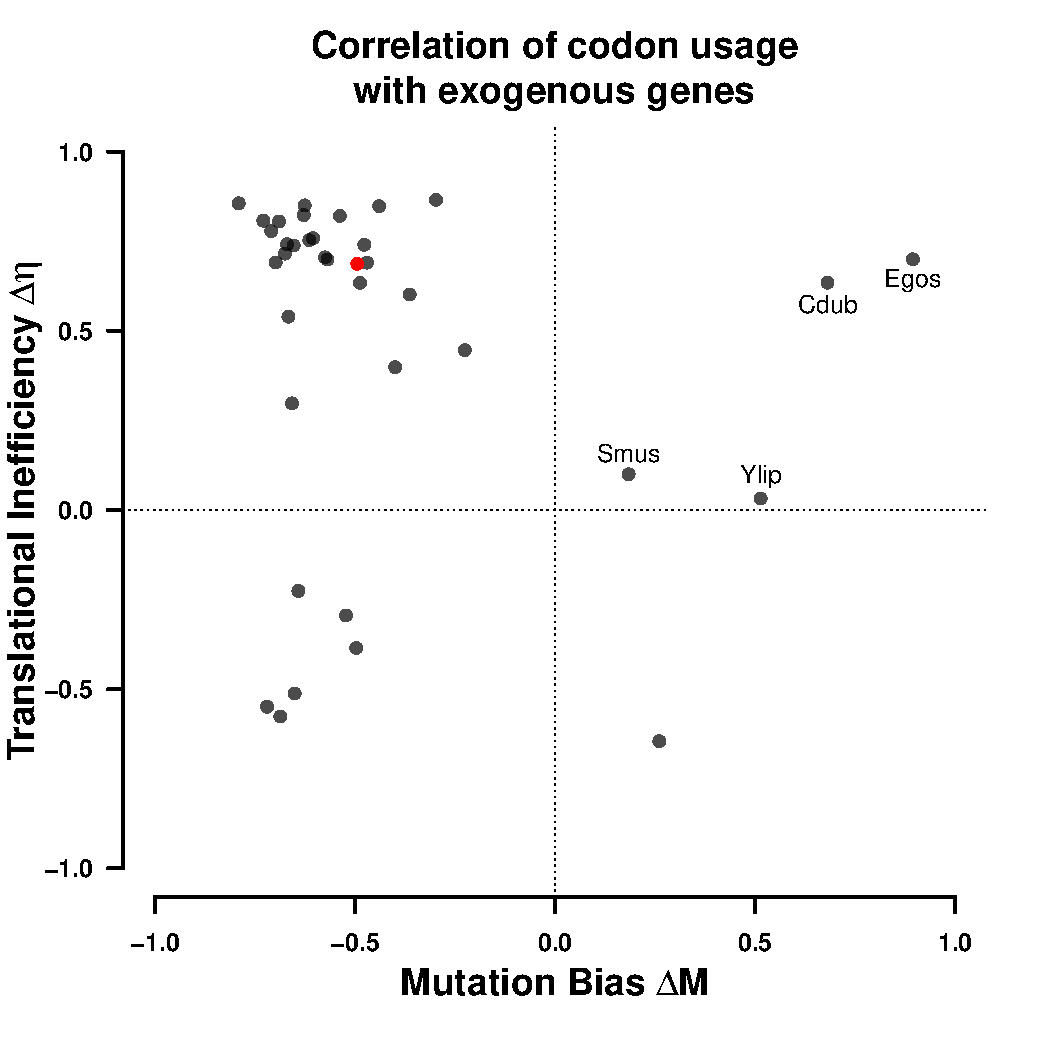
\includegraphics[width=0.5\textwidth]{ch3/csp_mean_correlation_exo.pdf}
	\caption{Correlation coefficient of \DM and \DE of the endogenous genes with 38 examined yeast lineages. 
	Dots indicate the correlation of \DM and \DE of the lineages with the endogenous and exogenous parameter estimates. 
	All regressions were performed using a type II regression line \citep{SokalAndRohlf1981}.}
	\label{fig:csp_endo_comp}
\end{figure}
\null
\vfill
\clearpage
\null
\vfill

\begin{figure}[h]
    \centering
    \begin{subfigure}
        \centering
        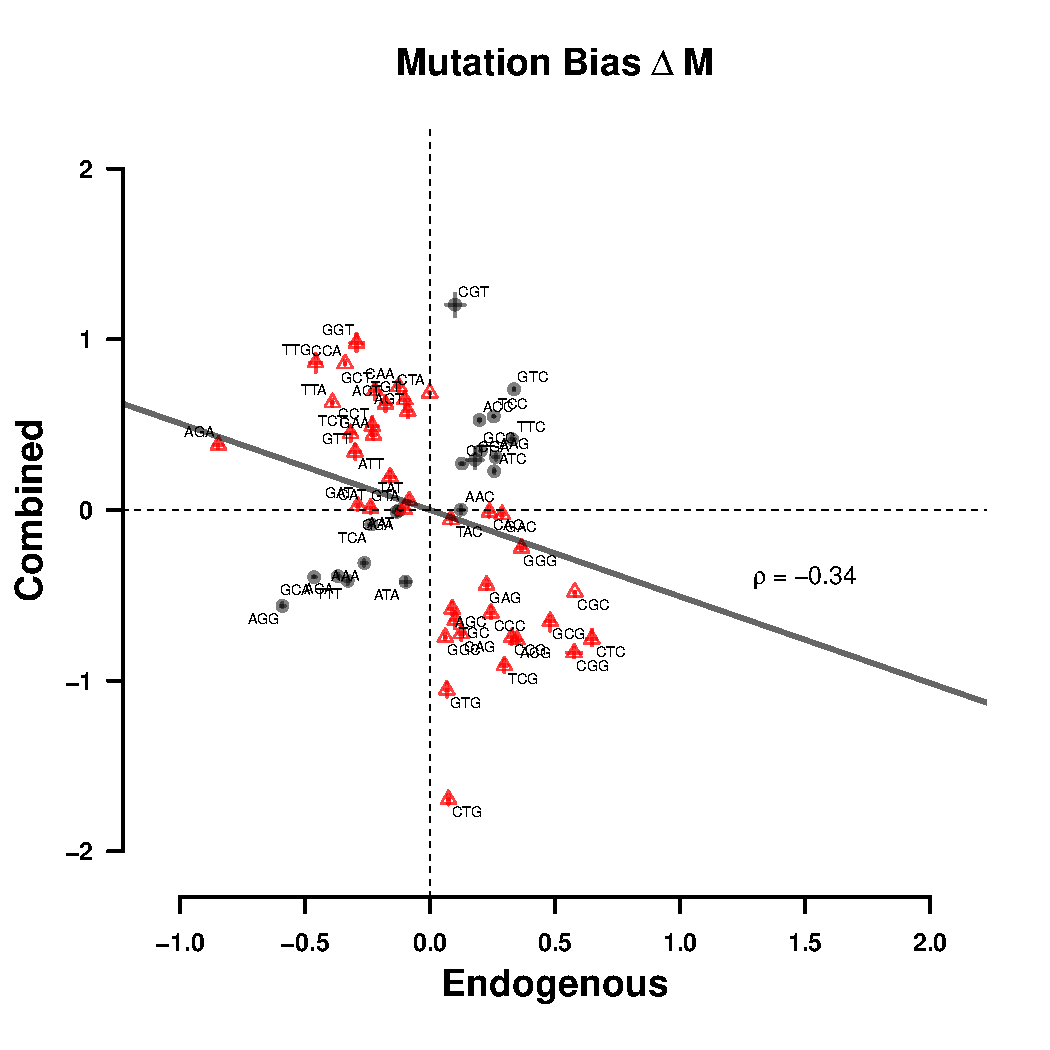
\includegraphics[width=.45\textwidth]{ch3/csp_corr_dm_full.pdf}
    \end{subfigure}
    \begin{subfigure}
        \centering
        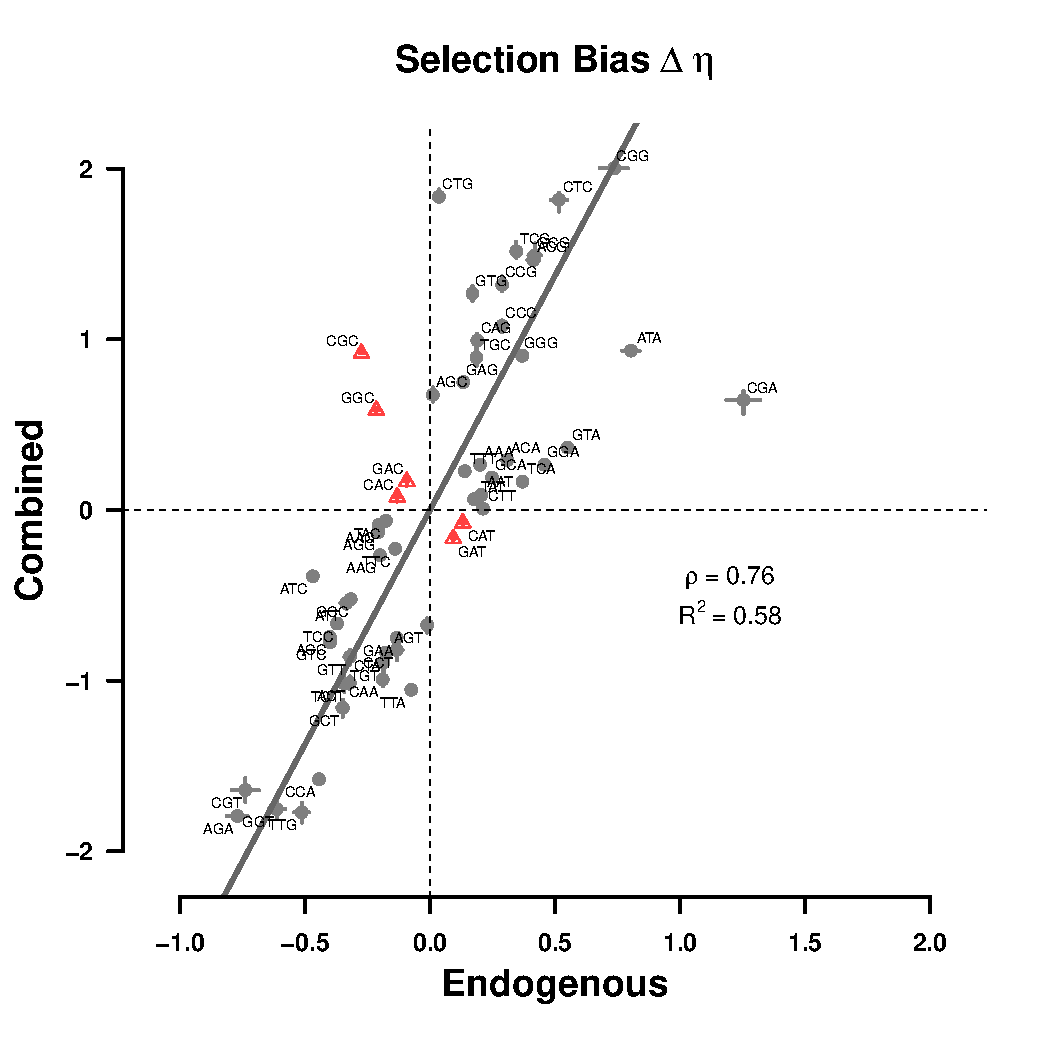
\includegraphics[width=.45\textwidth]{ch3/csp_corr_deta_full.pdf}
    \end{subfigure}
    \caption{Comparison of (a) mutation bias \DM and (b) selection bias \DE parameters for endogenous genes and combined gene sets.
      Estimates are relative to the mean for each codon family.
      Black dots indicate \DM or \DE parameters with the same sign for the endogenous and exogenous genes, red dots indicate parameters with different signs.
      Black line shows the type II regression line \citep{SokalAndRohlf1981}.
      Dashed lines mark quadrants.}
    \label{fig:csp_end_comb}
\end{figure}
\null
\vfill
\clearpage


\null
\vfill
\begin{figure}[H]
     \centering
	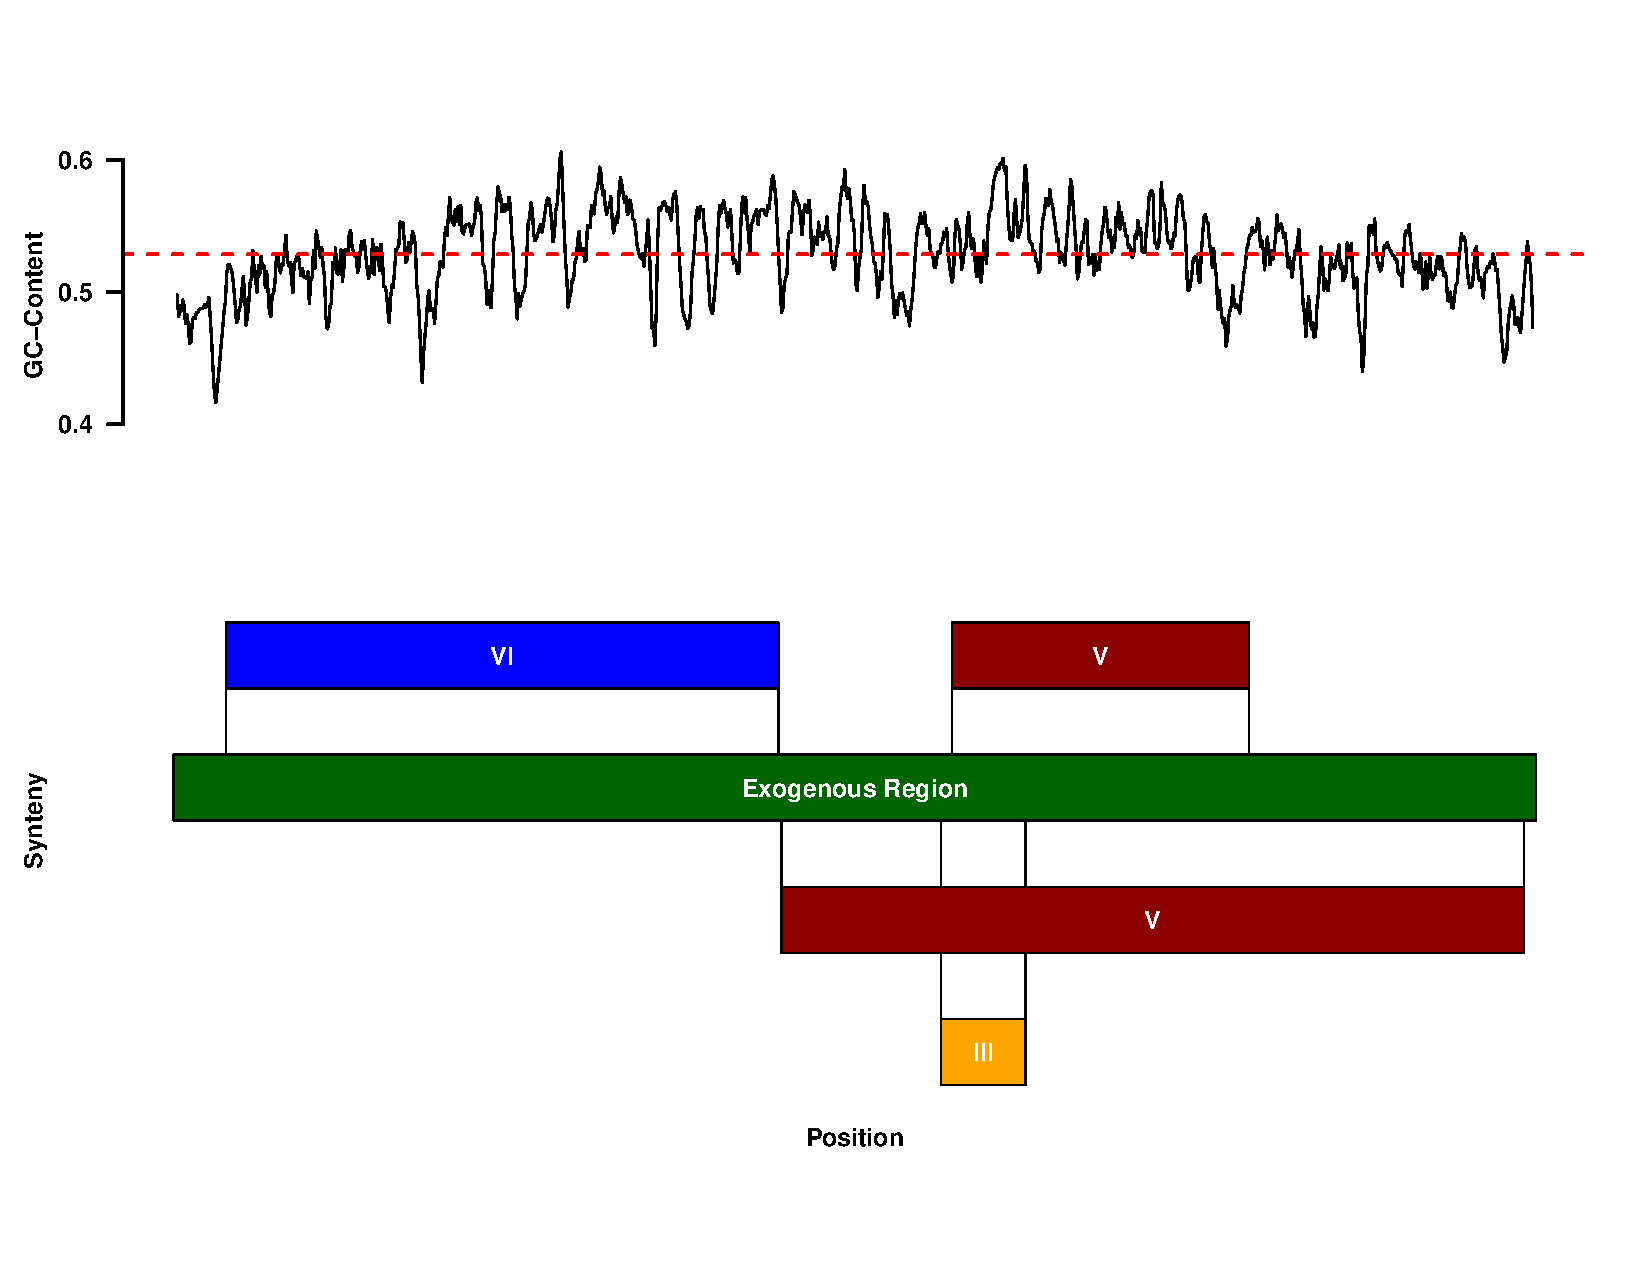
\includegraphics[width=0.8\textwidth]{ch3/synteny_blocks_and_gc.pdf}
	\caption{Synteny relationship of \gossypii and the exogenous genes. Indicated is the \GC along the introgression.}
	\label{fig:synt_rel}
\end{figure}
\null
\vfill
\clearpage
\null
\vfill
\begin{figure}[H]
     \centering
	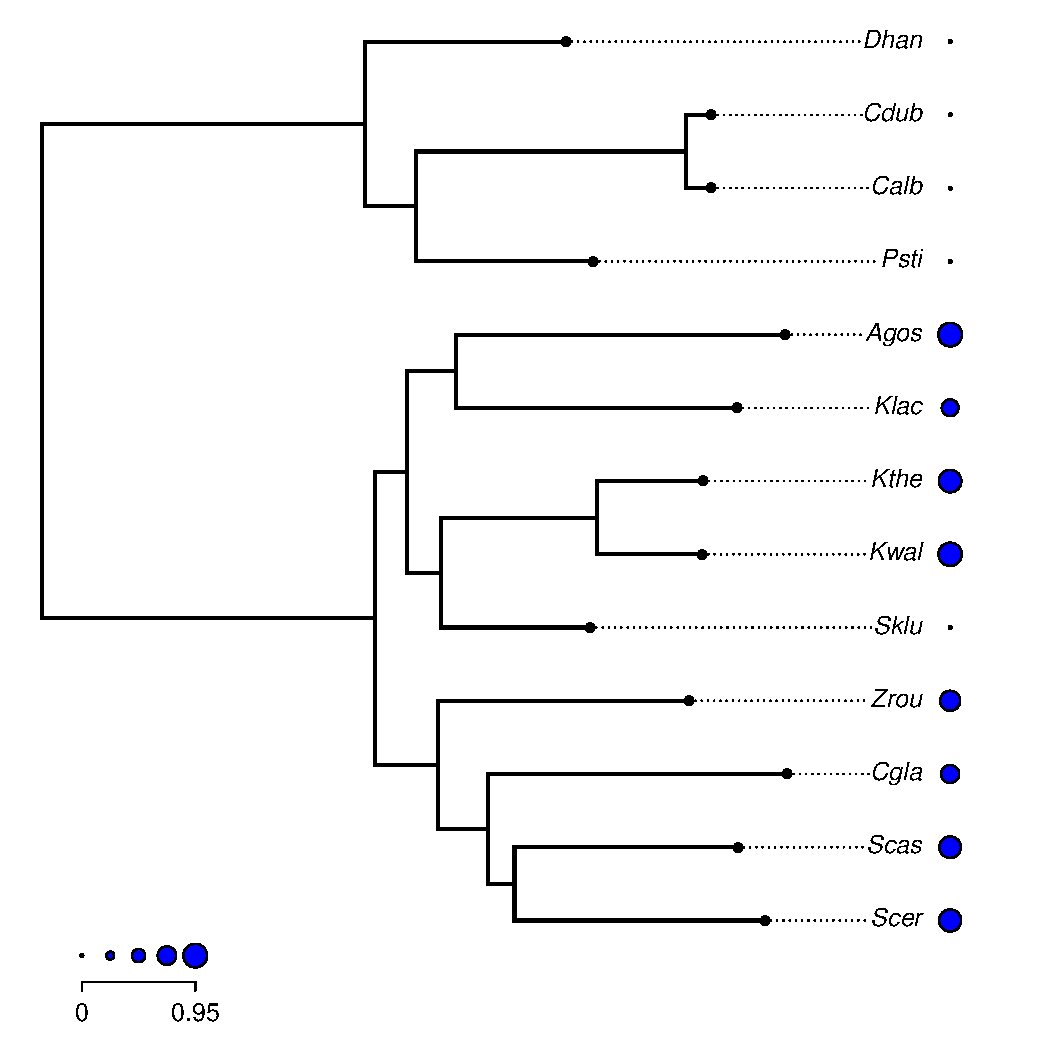
\includegraphics[width=0.8\textwidth]{ch3/synteny_coverage.pdf}
	\caption{Amount of synteny for each species in units of standard deviations for selected species.}
	\label{fig:synteny_species}
\end{figure}
\null
\vfill
\clearpage
\null
\vfill

\begin{figure}[h]
    \centering
    \begin{subfigure}
        \centering
        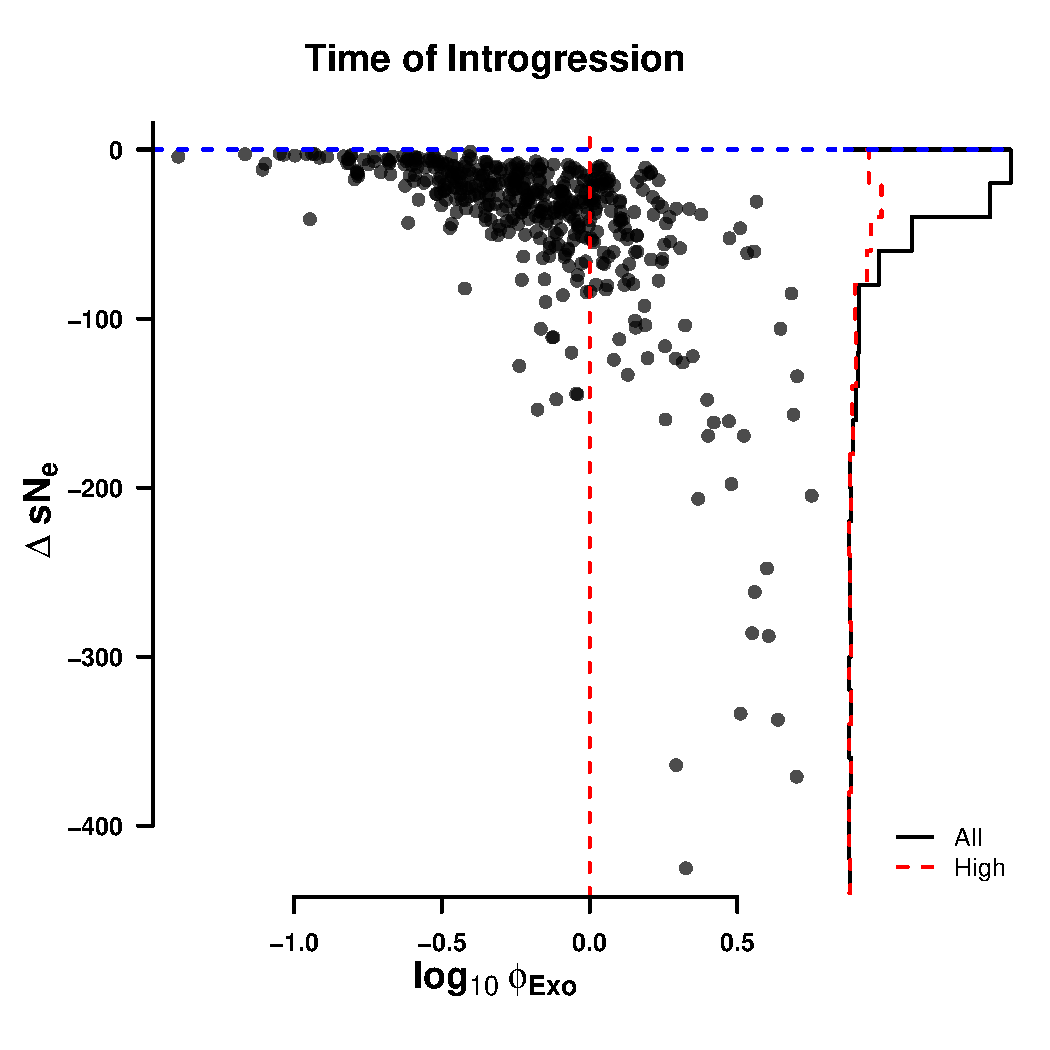
\includegraphics[width=.45\textwidth]{ch3/fitness_difference_gos_kappa1.pdf}
    \end{subfigure}
    \begin{subfigure}
        \centering
        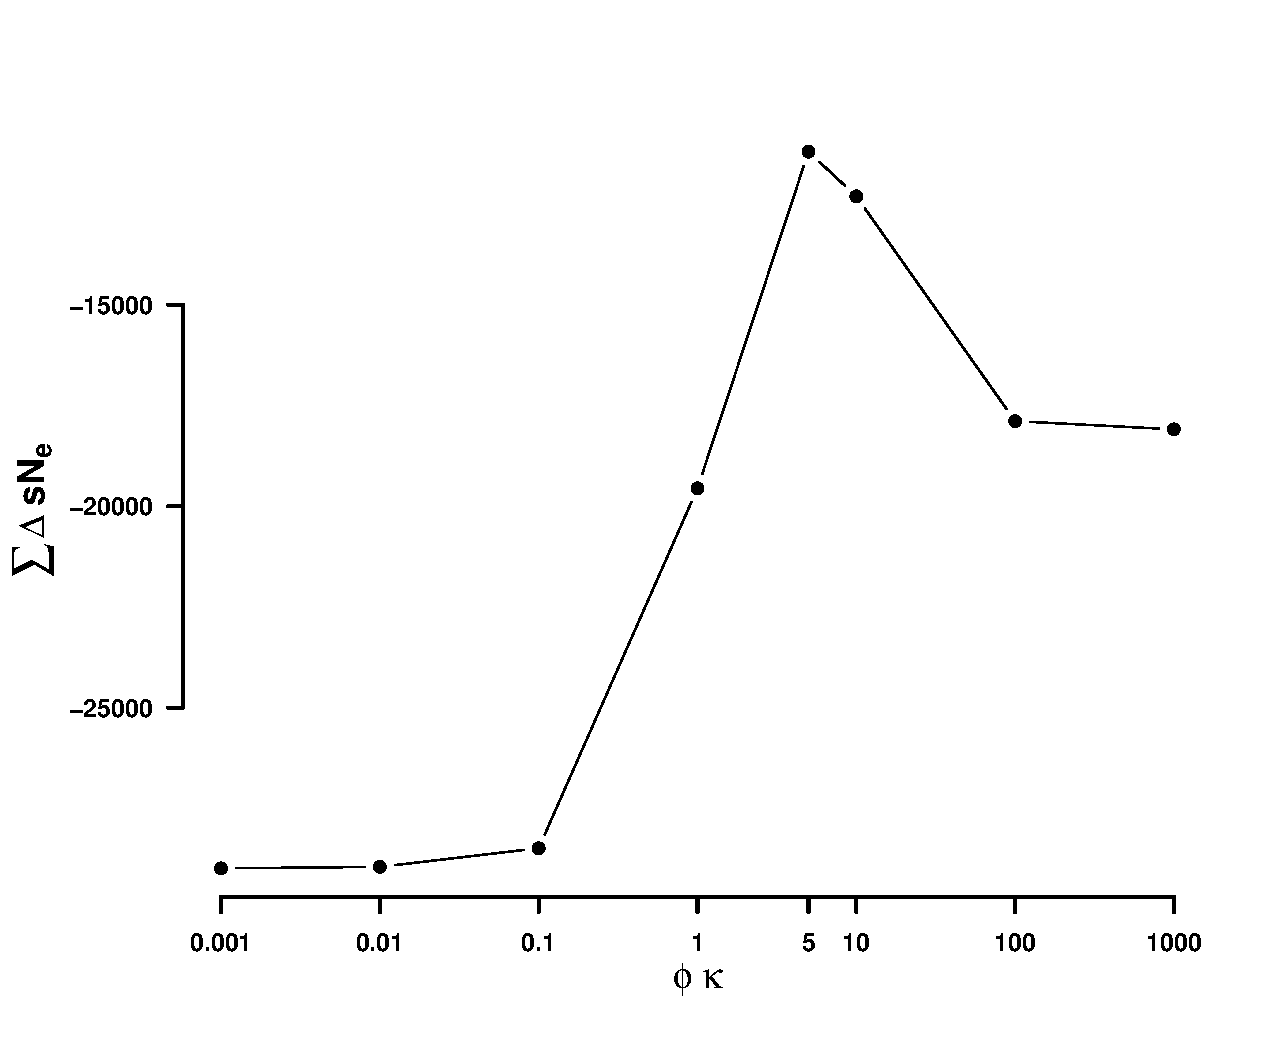
\includegraphics[width=.45\textwidth]{ch3/fitness_phi_scaling_gos.pdf}
    \end{subfigure}
    \caption{Genetic load (left) without scaling of $\phi$ per gene, and change of total genetic load with scaling $\kappa$ between \gossypii and \kluyveri (right)}
    \label{fig:sne_scaling}
\end{figure}
\null
\vfill
\clearpage
\null
\vfill
\begin{figure}[H]
     \centering
	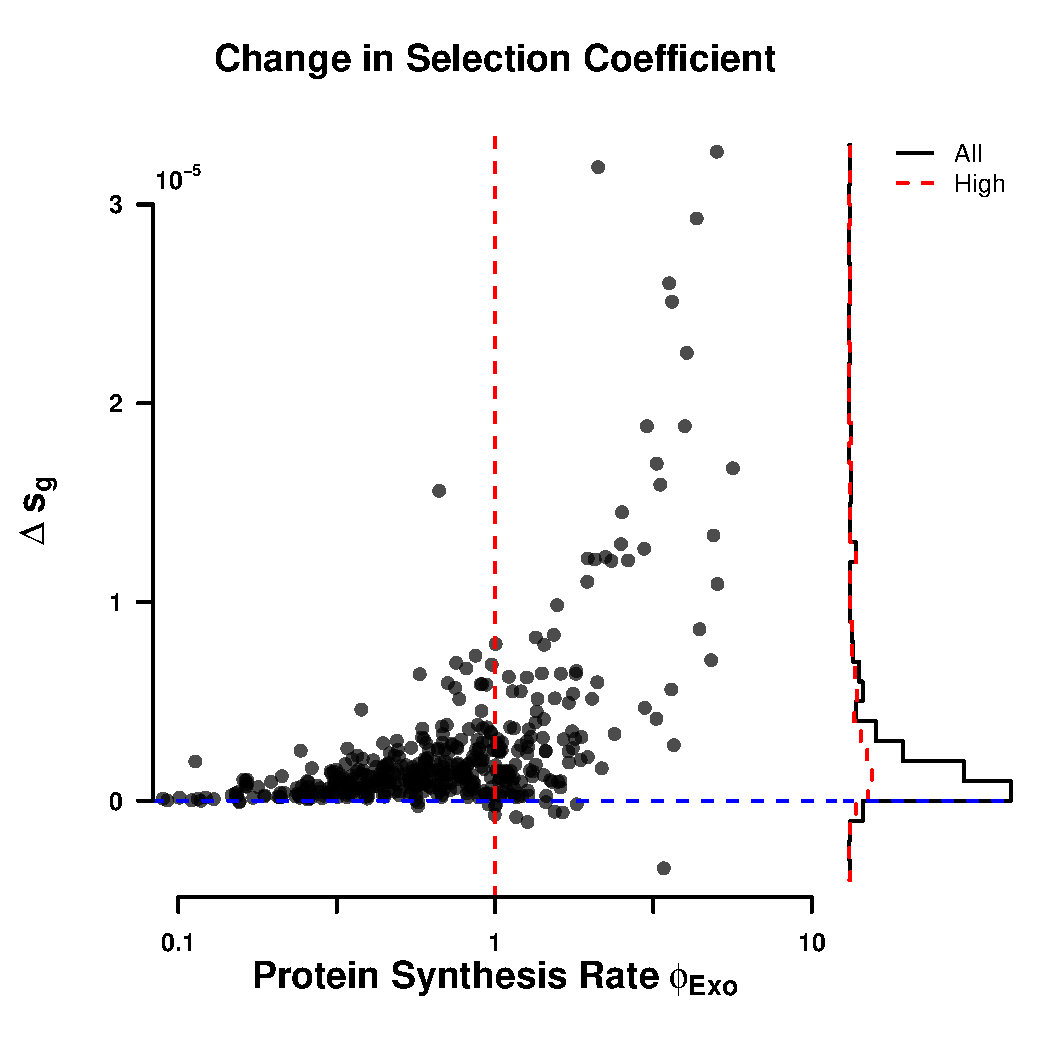
\includegraphics[width=.5\textwidth]{ch3/adaptation_total.pdf}
	\caption{Total amount of adaptation estimated to have occured between time of introgression and currently observed per gene.}
	\label{fig:adapt_tot}
\end{figure}
\null
\vfill
\clearpage

\begin{figure}[H]
     \centering
	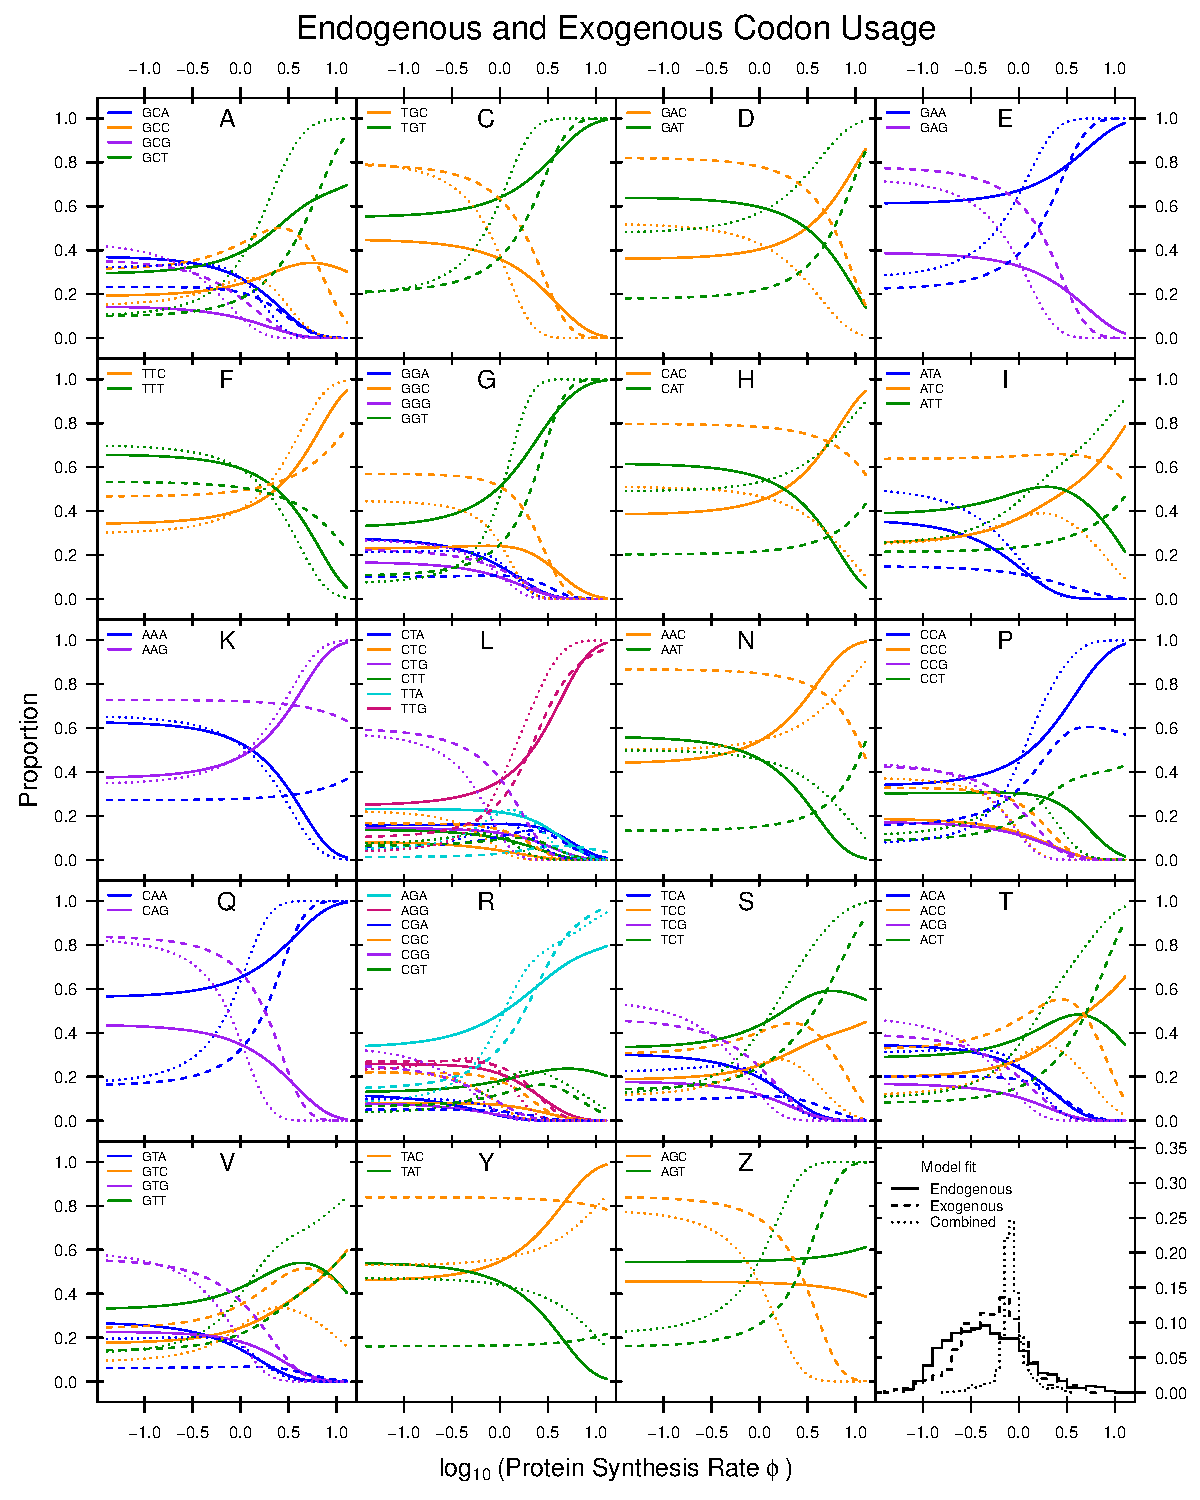
\includegraphics[width=0.9\textwidth]{ch3/CUB_cleft_main.pdf}
	\caption{Codon usage patterns for 19 amino acids. Amino acids are indicated as one letter code. 
	The amino acids Serine was split into two groups (S and Z) as Serine coded for by two groups of codons that are separated by more than one mutation.
	Solid line indicates the endogenous codon usage, dashed line indicates the exogenous codon usage, dotted line indicates the combined codon usage.}
	\label{fig:cub_all_sets}
\end{figure}
\doublespacing